%! Suppress = Ellipsis
\chapter[Graphical User Interfaces]{Getting Started with Graphical User Interfaces}\label{ch:starting-gui}

\section{Introduction}\label{sec:gui-introduction}
Building a \textbf{Graphical User Interfaces} (or GUI) may seem more complicated than it actually is. Once you learn the fundamentals, you can see that it's possible to put something together very quickly, especially if you already have some code to which to relate. In the previous chapter, you saw that you can control an experiment from the command line. It's possible to ask ourselves why going through the trouble of a user interface. In some cases, it can be very not only handy to control the parameters of an experiment and to monitor the output in a window especially designed, but it can become necessary to monitor the progress in real-time to make decisions while the experiment runs.

There are several options for building GUIs with Python. And in the community, there's no clear consensus on what is the best path to follow. For scientific applications, however, the only library which is powerful enough to achieve what you want to achieve is called \textbf{Qt}. Qt was developed as an application framework that allows developers to build apps that look native in different systems without changes to the code. Qt itself is a Finnish company with a long trajectory. It was part of Nokia for a while, and now they are publicly traded in the Helsinki exchange. It means that Qt is going to be around for a long time.

In this chapter, you're going to give the first steps for building a user interface using Qt, and the Python wrapper called \emph{PyQt}, that you installed in Chapter~\ref{ch:setting-up}. At Python, for the Lab, you've traditionally adopted PyQt, but in the past years, Qt itself took over the project called PySide, which is another wrapper for Qt. They are licensed under different open-source terms, and both are excellent. However, the structure of the PySide2 package is different from the PyQt package, and, for consistency, you keep using PyQt.

\checkInfo{Qt, PyQt, and PySide licensing}{If you're planning to release commercial software, or if you're packaging Qt, PyQt or PySide2 into your application, you should explore the different licensing options available.}


\section{Creating a Simple Window and Buttons}\label{sec:simple-window-andbuttons}
Now it's finally time to start using the empty folder from the M-\textbf{V}-C design pattern: the \textbf{View}. You start by learning how to create simple windows directly with Qt and proceed to a fully-featured user interface for our experiment. You start just with scripts, and you slowly grow in complexity.

The best way to get started with Qt is with a quick example. You can create a new file, \textbf{simple\_window.py} in the \emph{Examples} folder, with this code:

\begin{minted}{python}
    from PyQt5.QtWidgets import QApplication, QMainWindow

    app = QApplication([])
    win = QMainWindow()
    win.show()
    app.exec()
\end{minted}

You will come back to the code above over and over again. In the beginning, it's hard to remember, but once you do it often enough, it sticks. After importing, you create a \py{QApplication}, a \py{QMainWindow}, you show it, and you run the app. This code should produce a very simple window that looks like the image below:

\begin{center}
    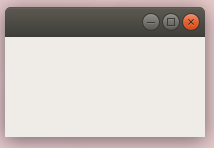
\includegraphics[width=.3\textwidth]{images/Chapter_08/01_simple_window.png}
\end{center}

The style matches the operating system where it runs. It's a simple, empty window. However, you can already start understanding how Qt works. A user interface is a program that keeps running in a loop. When you click and drag to resize a window, for example, there's always a program responsible for knowing how to do it. In Qt, this never-ending loop is the \py{QApplication}. Whatever window you want to create needs to belong to an application, and that is why the first thing you did was defining \py{app}.

In the following line, you define a new object, called \py{win}, which is a \py{QMainWindow}. As the name suggests, the main windows are the core of the user interface. From the main window, you can open dialogs, other windows, but the main window is central to our program. After creating it, you show it. The last line is where the application loop starts. The \py{app.exec()} command is blocking. Therefore nothing that comes after is executed until you finish with the user interface.

\questionInfo{Exercise}{To understand a bit better what is going on with the user interface, you're encouraged to try different things. For example, what happens if you don't show the window or add a few print statements to see when they get executed. You can also try to define the window before the application.}

Having an empty window is not particularly useful, so you can start adding elements to it. First, you add a title to the window, like this:

\begin{minted}{python}
    win.setWindowTitle('My First Window')
\end{minted}

Very slowly, our program starts taking shape and looking more professional. You can also add an interactive element, such as a button. You can define one like this:

\begin{minted}{python}
    from PyQt5.QtWidgets import QApplication, QMainWindow, QPushButton

    app = QApplication([])
    win = QMainWindow()
    win.setWindowTitle('My First Window')
    button = QPushButton('Press Me', win)
    win.show()
    app.exec()
\end{minted}

Which will produce a small window, like this:

\begin{center}
    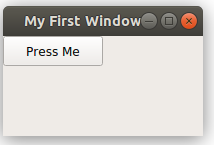
\includegraphics[width=.3\textwidth]{images/Chapter_08/02_simple_window_and_button.png}
\end{center}

Notice that when you defined the button, you added a second argument, \py{win}. Qt has a hierarchical structure, where each element is called a \emph{widget}. You've imported three widgets so far: the application, the window, and the button. All widgets live inside the application loop, but you've to establish the relationship between them. By passing the window as the second argument, you're explicitly saying that the button belongs to the window.

\questionInfo{Exercise}{Remove the \py{win} from the definition of the button, and see what happens}
\questionInfo{Exercise}{Alter the order and make the button the parent of the main window, does this work?}

A big part of working with Qt is finding out how to relate different widgets to each other, how to position them. \py{QMainWindows} are special because they must hold widgets within them. That is why they specify a method to determine which Widget is the most important for the window, or in Qt jargon, which Widget is the central Widget. You can explicitly declare it:

\begin{minted}{python}
    button = QPushButton('Press Me')
    win.setCentralWidget(button)
\end{minted}

You removed the \py{win} from the declaration of the button, but if it's there it doesn't change the behavior. The window now looks somewhat different:

\begin{center}
    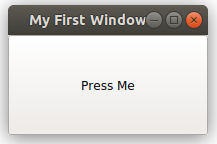
\includegraphics[width=.3\textwidth]{images/Chapter_08/03_simple_window_and_central_widget.png}
\end{center}

You can try resizing the window, and you see that the button scales. By declaring the button as the central Widget of the window, you made the relationship even stronger. The last possibility which is worth mentioning before moving forward is that you can also show the button independently from the window, like this:

\begin{minted}{python}
    win.setWindowTitle('My First Window')
    button = QPushButton('Press Me')
    win.show()
    button.show()
\end{minted}

In this case, the window and the button are two independent components, like you show in the image below. For the program to finish, you must close both the button and the window.

\begin{center}
    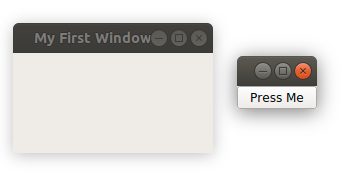
\includegraphics[width=.3\textwidth]{images/Chapter_08/04_window_button_separated.png}
\end{center}

Qt offers a great deal of flexibility, which doesn't mean you need actually to use it. Having buttons floating around the screen does not sound like a good idea, but it's a possibility in case you ever need it.

Now that you've a button on a window, you're craving to do something with it.


\section{Using Signals and Slots}\label{sec:signals-slots}
Qt offers a programming pattern known as \emph{Signals} and \emph{Slots}. The core idea is that different actions on a user interface trigger a signal. For example, moving the mouse over an element triggers a signal. This signal is then caught by \emph{slots}, which do something with the information provided. When you move the mouse over a button (this is also knowns as hovering), its background changes color. It's a clear example of the signal/slot paradigm.

Every Widget that you can place on screen has a myriad of signals. From interactions with the mouse to changes in shape or size triggered by reshaping the window, to time-based signals. It does not mean you need to know them all, nor that you use them all. But once you understand the pattern, you know where to go and find what you're after. The button has one signal called, very eloquently, \py{clicked}. To use it, you must define a function that can be called every time the signal fires. This function is the \emph{slot}. You can expand our example code like this:

%! Suppress = Ellipsis
\begin{minted}{python}
def button_clicked():
    print('Button Clicked')

[...]
button = QPushButton('Press Me')
button.clicked.connect(button_clicked)
win.setCentralWidget(button)
\end{minted}

You can see that every time you click the button, the program prints a message to the screen. It's very important to note that you used \py{button_clicked} and not \py{button_clicked()}. It's the same that you discussed in Section~\ref{subsec:multithreading} when discussing multithreading. You must use the function itself as a slot, and not the outcome of the function.

\subsection{Starting a scan}\label{subsec:start-scan-gui}
With what you've done so far, triggering a scan from the user interface becomes almost trivial. For the time being, you can keep working on the \emph{Examples} folder, but this time let's create a new file called \textbf{start\_gui.py}. You only need that when you press the button, a scan starts. You need to mix what you already have in \textbf{run\_experiment.py} with what you've done above. It can look like this:

\begin{minted}{python}
    from PyQt5.QtWidgets import QApplication, QMainWindow, QPushButton

    from PythonForTheLab.Model.experiment import Experiment

    experiment = Experiment('experiment.yml')
    experiment.load_config()
    experiment.load_daq()

    app = QApplication([])
    win = QMainWindow()
    win.setWindowTitle('My First Window')
    button = QPushButton('Start Scan')

    button.clicked.connect(experiment.do_scan)

    win.setCentralWidget(button)
    win.show()
    app.exec()

    experiment.finalize()
\end{minted}

The code above is a merge between what you did in the previous chapter and this one. You define the experiment as always, and the window and button as you've just learned. However, the line that does all the magic is this one:

\begin{minted}{python}
    button.clicked.connect(experiment.do_scan)
\end{minted}

You can try the program. When you click the button, a scan starts. However, there's something else happening. The window freezes, you're not able to reshape it, close it. In some cases, especially on Windows, the program crashes, and you get a message saying whether you want to report the issue.

\questionInfo{Exercise}{Can you guess why the window freezes?}

When you described the flow of a Qt program, you talked about a loop taking care of the interactions within the program. However, if you trigger a scan using \py{do_scan}, you're going to block that loop. Both Qt and Python are single-threaded applications by default, and when one blocks, the other blocks as well. And by talking about single-threaded applications, you gave a hint to how this can be solved.

At the end of the last chapter, you developed a different method called \py{start_scan} that creates a separate thread to hold the scanning, effectively releasing the main thread to do other tasks. You can change just one line of code and achieve a very different behavior:

\begin{minted}{python}
    button.clicked.connect(experiment.start_scan)
\end{minted}

You've developed a somewhat functional program. You've a window with a button from which you can control our experiment. It's already quite an excellent achievement. You also got some extra features out of the box, such as preventing the user from triggering two scans at the same time.

Sometimes, the easiness of developing this kind of solution misguides the readers. It was so easy to achieve what you achieved so far because you spent a lot of time and effort developing a proper \emph{experiment class}. The threading, the checks to prevent two scans, and some extra things that keep appearing in this and next chapter are thanks to a well-designed model.


\section{Extending the Main Window}\label{sec:extending-main-window}
You've seen how to get started by creating the main window and adding a button to it. However, you can also start seeing that if you try to add more elements, the code is going to become more and more convoluted. It would be a nice addition if the window you design here could be used for different purposes as well. As you've already seen many times, a good idea when you want to make blocks of code reusable is to convert them into classes. Qt is ideally suited for this because every Widget they provide is an object with a special inheritance tree.

In the folder \emph{View} you can create a file called \textbf{main\_window.py}, and you can add the following code:

\begin{minted}{python}
    from PyQt5.QtWidgets import QMainWindow


    class MainWindow(QMainWindow):
        def __init__(self):
            super().__init__()
            self.setWindowTitle('My First Window')
\end{minted}

Before discussing what you've done, you can quickly go back to \textbf{start\_gui.py} and change the following two lines of code:

\begin{minted}{python}
    win = QMainWindow()
    win.setWindowTitle('My First Window')
\end{minted}

with this one:

\begin{minted}{python}
    win = MainWindow()
\end{minted}

You should also remember to change the imports at the top of the file by these:

\begin{minted}{python}
    from PyQt5.QtWidgets import QApplication
    from PythonForTheLab.View.main_window import MainWindow
\end{minted}

If you run the code, you see that it behaves as it was behaving previously. In our code, you create a new class called \py{MainWindow}, which in turn inherits from \py{QMainWindow}. It's always important to call \py{super()} because that runs the init method from the QMainWindow itself, setting up all the parameters, signals, properties that you need to generate a window. There is, however, a difference with a plan \py{QMainWindow}, you specify its title. Effectively, you've now extended the pure \py{QMainWindow} class to include a title by default.

\checkInfo{Naming conventions}{It's a personal preference when I start developing a program that has only one main window to name it \py{MainWindow}, removing the preceding \py{Q}. It can lead to mistakes if you overlook the small difference in both names. Depending on taste, an alternative is to call the windows by what they are supposed to do, such as \py{ScanWindow}. It depends on the reader's preferences.}

You can add the button, and the slot, like this:

\begin{minted}{python}
from PyQt5.QtWidgets import QMainWindow, QPushButton


class MainWindow(QMainWindow):
    def __init__(self, parent=None):
        super().__init__(parent=parent)
        self.setWindowTitle('My First Window')
        self.button = QPushButton('Press Me')
        self.setCentralWidget(self.button)

        self.button.clicked.connect(self.button_clicked)

    def button_clicked(self):
        print('Button Clicked')
\end{minted}

You can test this code again and see that you've recovered what you had before. Every time you press on the button, a message appears on the screen. You can also go one step further and start thinking about how to work with the experiment itself. The window is not aware of any experiments, but you would like to be able to trigger a scan if you press the button. Therefore, the experiment has to come from outside of the class and be stored within.

You've already done something like this. When you developed the driver in Section~\ref{sec:going-higher-level}, you could send the port number to the class through the \py{__init__} method. You did the same for the device model in Section~\ref{sec:device-model}, and for the experiment model in Section~\ref{sec:skeleton-experiment-model}. In all those cases, you were using simple strings, but you're not limited to them. Arguments of methods, or any function for the matter, can be complex objects as well.

You can adapt the \py{MainWindow} to accept an experiment as argument, store it as an attribute and use it when you need to. The code would look like this:

\begin{minted}{python}
    [...]
    class MainWindow(QMainWindow):
        def __init__(self, experiment=None):
            super().__init__()
            self.experiment = experiment

            [...]
        def button_clicked(self):
            self.experiment.start_scan()
            print('Scan Started')
\end{minted}

The changes to the code were minimal but significant. You've included \py{experiment=None} in the init. You've provided a default value for the experiment because this allows us to run the program even if you've no experiment defined. It's useful if you want to test how the window looks like quickly. However, as soon as you press the button, the program crashes. You've to update the \textbf{start\_gui.py} script to accommodate for the changes:

\begin{minted}{python}
experiment = Experiment('experiment.yml')
experiment.load_config()
experiment.load_daq()

app = QApplication([])
window = MainWindow(experiment)
window.show()
app.exec()

experiment.finalize()
\end{minted}

You pass \py{experiment} directly to the window, and it takes care of the rest. You can now safely trigger a scan from the user interface. What is important to note is that once you reach this step, all the rest happens directly on the view. The script that you use to open the window stays unaltered. Even in much more complex programs, you use the same pattern\footnote{See, for example, how PyNTA starts its user interface: https://bit.ly/WindowExperiment}.

\section{Adding Layouts}\label{sec:adding-layouts}
So far, our window holds only one button, and you set that button to be the central Widget of the window. This makes it virtually impossible to add any other button or object. Therefore, it's time to start sophisticating our user interface\footnote{In this chapter you decided to go lower level, programming every feature, but in the next chapter you will see how to do it with the QtDesigner software, which will speed up the process}. The basic building blocks in Qt are \py{QWidgets}, and Qt allows us to place widgets inside of widgets at our will. You also know that Main Windows require a central widget. Therefore, you can create a widget that holds two buttons: start and stop, and that Widget is the central Widget of the window. You use this opportunity to clean up the names you've used, to make them more descriptive as well, it's important to pay attention to all the changes made:

\begin{minted}{python}
from PyQt5.QtWidgets import QMainWindow, QPushButton, QWidget


class MainWindow(QMainWindow):
    def __init__(self, experiment=None):
        super().__init__()
        self.experiment = experiment
        self.setWindowTitle('Scan Window')

        self.button_widgets = QWidget()
        self.start_button = QPushButton('Start', self.button_widgets)
        self.stop_button = QPushButton('Stop', self.button_widgets)

        self.setCentralWidget(self.button_widgets)

        self.start_button.clicked.connect(self.start_scan)

    def start_scan(self):
        self.experiment.start_scan()
        print('Scan Started')
\end{minted}

If you run the program again, you will see a Window like the one below:

\begin{center}
    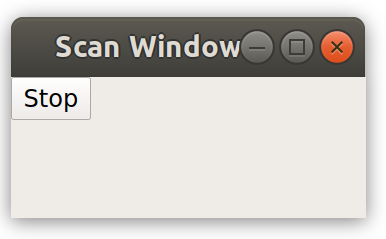
\includegraphics[width=.3\textwidth]{images/Chapter_08/05_window_without_layout.png}
\end{center}

The stop button is visible, but not the start button. It happens because Qt has no way of knowing where you want to add the buttons and place them in the same position. The one that gets added later is on top.

\questionInfo{Exercise}{Change the order in which you define the buttons and see that one or the other gets on top. If the button that is below has a much longer text, you can see it beneath the top one.}

You could specify explicit coordinates for the positions of the buttons, but there's a much simpler approach using layouts. In Qt, there are 4 basic layout types: Horizontal, Vertical, Grid, and Form. With the first two, each time you add a widget, it's added either below or to the right. With the grid layout, you can control the position, width, and height based on a grid you define. The form defines two columns, ideally to hold some labels and inputs. You see more about layouts in the following chapter. For the time being, if you want to add two buttons, you can choose a horizontal layout. The code of the \py{MainWindow} takes a few extra lines to set everything up properly:

\begin{minted}{python}
from PyQt5.QtWidgets import QHBoxLayout
[...]
self.button_widgets = QWidget()
self.start_button = QPushButton('Start')
self.stop_button = QPushButton('Stop')
layout = QHBoxLayout(self.button_widgets)
layout.addWidget(self.start_button)
layout.addWidget(self.stop_button)

self.setCentralWidget(self.button_widgets)
\end{minted}

In Qt, the horizontal layout is called \py{QHBoxLayout}, and you apply it to the \py{buttons_widget}. Then, you add the start and stop to the layout, instead of directly to the widget. This window will look much better:

\begin{center}
    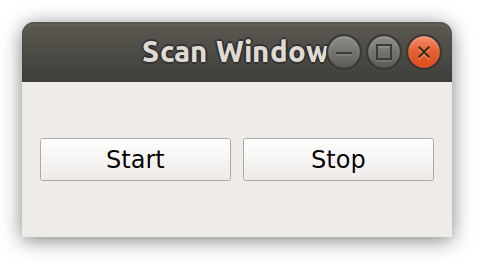
\includegraphics[width=.3\textwidth]{images/Chapter_08/06_window_with_layout.png}
\end{center}

If you resize it, you see that the buttons take the entire width, and they are always centered. It's already a good improvement compared to the simple window with which you started. Before you finish this section, these two exercises are a good way of practicing the skills acquired so far:

\questionInfo{Exercise}{Change \py{QHBoxLayout} by \py{QVBoxLayout} to see the buttons stacked vertically.}

\questionInfo{Exercise}{Connect the stop button to a method that stops the scan}

\section{Plotting Data}\label{sec:plotting-data}
You finish this section by adding a plot of the data in real-time. You already did something similar in Section~\ref{sec:basic-plotting}. Parts of the code are very similar. Our window slowly starts getting more complex, with more elements. So far, you've two buttons stacked horizontally, but you would like to show the plot beneath the buttons, not next to them. One of the most natural solutions is to start stacking widgets, instead of making the \py{buttons_widget} the central Widget, you can make another one that contains the buttons and the plot.

\begin{minted}{python}
import pyqtgraph as pg
from PyQt5.QtWidgets import (QMainWindow,
                             QPushButton,
                             QWidget,
                             QHBoxLayout,
                             QVBoxLayout, )

class MainWindow(QMainWindow):
    def __init__(self, experiment=None):
        super().__init__()
        self.experiment = experiment
        self.setWindowTitle('Scan Window')

        self.central_widget = QWidget()
        self.button_widgets = QWidget()
        self.start_button = QPushButton('Start')
        self.stop_button = QPushButton('Stop')
        self.plot_widget = pg.PlotWidget(title="Plotting I vs V")
        self.plot = self.plot_widget.plot([0], [0])

        layout = QHBoxLayout(self.button_widgets)
        layout.addWidget(self.start_button)
        layout.addWidget(self.stop_button)

        central_layout = QVBoxLayout(self.central_widget)
        central_layout.addWidget(self.button_widgets)
        central_layout.addWidget(self.plot_widget)

        self.setCentralWidget(self.central_widget)
\end{minted}

Some remarks about the code before you run it. You're using \py{()} for the import because it makes it easier to stack the modules instead of having a very long line that becomes hard to read. In the window, you define three widgets now, \py{central_widget}, \py{button_widgets}, and \py{plot_widget}. The plot widget is very similar to what you did in the previous chapter. The only difference is that you store the Widget itself and the plot separately, and you explain why later. You didn't touch the buttons, but instead of adding them as the central Widget, you add them to a higher-order widget. By stacking the buttons horizontally between themselves, but vertically to the plot, you get a window that looks like this:

\begin{center}
    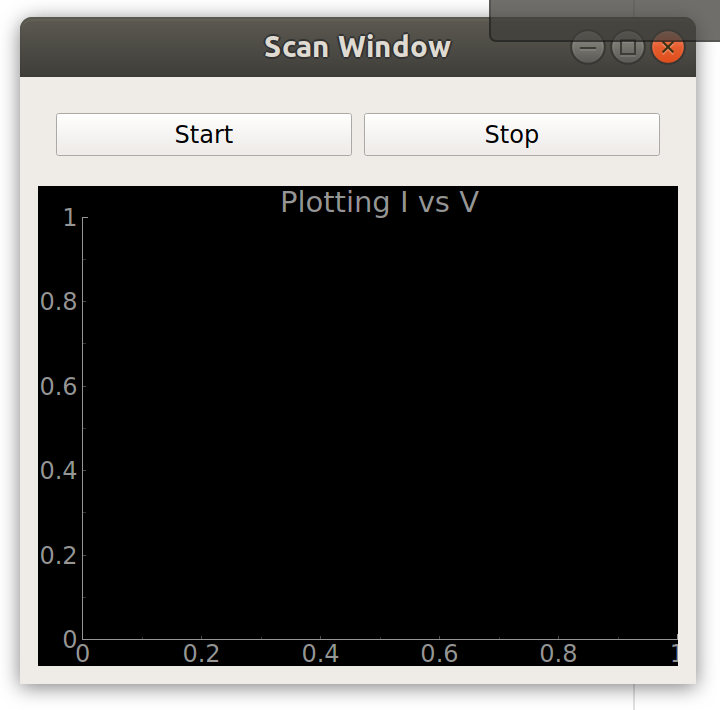
\includegraphics[width=.4\textwidth]{images/Chapter_08/07_window_empty_plot.png}
\end{center}

You're halfway through with what you wanted. If you resize the window, the plot changes, taking all the space available, even if you expand the window vertically, there's no gray area around the buttons. How the surrounding elements control the shape of a widget is one of the properties that can be specified.

\tipsInfo{Qt options}{You make several remarks about possibilities with Qt that you don't explore further. You just want to point out that every single thing that happens on a user interface was decided, and can be changed. Not only the aspect, such as colors but also how different elements relate to each other and change shapes when the container window changes.}

To plot the data you acquire, you just need to update the plot periodically. Qt offers a special object called \py{QTimer} that also specifies signals. With timers, you can trigger periodic actions without interrupting the rest of the program. You also need to develop a method that can update the plot. The Main Window code looks like this:

\begin{minted}{python}
    from PyQt5.QtCore import QTimer
    [...]

    class MainWindow(QMainWindow):
        def __init__(self, experiment=None):
            [...]
            self.timer = QTimer()
            self.timer.timeout.connect(self.update_plot)
            self.timer.start(50)

        def update_plot(self):
            self.plot.setData(self.experiment.scan_range, self.experiment.scan_data)
\end{minted}

The timer is relatively easy to understand. It's an object that triggers a signal, \py{timeout} periodically. You connect that signal to the method \py{update_plot}. When you start the timer, you need to specify the time interval in milliseconds, therefore $50\,\textrm{ms}$ means a refresh rate of $20\,\textrm{Hz}$. The \py{update_plot} method is different from what you did in the previous chapter. Instead of using \py{plot}, you're using \py{setData}. There are two reasons for it. First, if you use \py{plot()}, you create a new plot on top of the existing one. You wouldn't be refreshing the data but drawing on top of it. After a while, especially if the parameters or results change, you would see several lines overlapping. The second reason is speed. \py{plot()} is a relatively slow method because several things need to be set up, such as the axes, labels, ticks. By using \py{setData} PyQtGraph automatically reuses the elements available.

However, if you try to run the code, you will get a problem:

\begin{minted}{bash}
    AttributeError: 'Experiment' object has no attribute 'scan_range'
\end{minted}

\questionInfo{Exercise}{Find out why are you getting this error even though you didn't find it when running a more straightforward script in the previous chapter}

When the window starts, you automatically start the timer, which, in turn, tries to update the plot. However, the experiment class does not have any \py{scan_range} nor \py{scan_data} until the experiment starts running. A bypass to the problem would be to start the timer after you've started the scan, but this is very unreliable. Best-practices in Python indicate that you should always define attributes in classes in the \py{__init__} method. It means that as soon as you create the object, the attributes exist, even if with place-holder values.

When you developed the \emph{Experiment class}, you completely neglected this practice. You added \py{self.} whenever you needed to have data available through the class and also from outside of it. You leave the definition of most of the attributes to the reader, but you show how to solve the problem with the scan. Going back to the experiment model, you need to add the following:

\begin{minted}{python}
    class Experiment:
        def __init__(self, config_file):
            [...]
            self.scan_range = np.array([0]) * ur('V')
            self.scan_data = np.array([0])  * ur('V')
\end{minted}

You decided to define both attributes as numpy arrays holding only one value: $0\,\textrm{V}$. If you try to plot these results, you get a single point at the origin. It may raise other questions, such as whether it's better to have a $0$ or a \py{None} value, because $0\,\textrm{V}$ could be a valid measured value. It's left to the sensitivity of the reader to judge what is best in their specific case. For our purposes, this is enough to get the window running and showing a plot of the data in real-time once the scan starts.

\questionInfo{Exercise}{Every attribute in any class should be defined in the init of that class. Go through all the models, and see whether there are attributes used but not defined at instantiation.}

\subsection{Increasing the refresh rate and number of data points}\label{subsec:refresh-rate-and-number-of-data-points}
When you follow the strategy of using a timer for refreshing the plot, you can be tempted to increase the refresh rate to make the animations more appealing, but you've to be careful with this. On the one hand, if you're generating data at, let's say, $1\,\textrm{Hz}$, doesn't matter how fast you refresh the plot, it won't change faster than once per second.

Let's assume you're acquiring data much faster than once per second, perhaps at hundreds or thousands of new points per second. You've to consider how fast the screen of the computer can redraw the elements on it. Most screens work at $30\,\textrm{Hz}$, some may go to $60\,\textrm{Hz}$. Therefore, if you try to update the plot faster than that, you just waste computer power on something that the screen never can show us.

There's one additional limitation that is our own eyes. You can't process images faster than at 30fps. Already at $50\,\textrm{Hz}$, you don't see the lights in our room blinking. If you're not interested in video quality for the update of our plots, you can safely go down to $20\,\textrm{Hz}$, and the images still look fluid.

\questionInfo{Exercise}{Instead of plotting data from the device, you can update the plot with points that oscillate in time and see up to which point the refresh rate affects the quality of what you're showing.}

There's one more thing to consider beyond the refresh rate, which is the number of points you're plotting. Most screens have a few thousand pixels in each direction. A very common resolution is $1920\times1440\,\textrm{pixels}$. If you acquire $10000$ data points and try to show them on the screen, they have to be reduced almost 5 times to fit the number of pixels available on the screen. In this reduction process, you can lose many details. If you use downsampling, for example, and you're looking for a narrow peak, the chances of it appearing on the image can be very little.

You've to be aware of the number of data pixels that you try to show not only on user interfaces but also when you're preparing plots for printing or inserting into a PDF. The number of dots a printer can generate is normally specified as dots per inch, or dpi. Even at $600\,\textrm{dpi}$, an image with a width of $8\,\textrm{cm}$ (standard 1-column figure on a paper) will have under 2000 dots in its horizontal direction. And, of course, a reader behind a computer screen is limited to its pixels.

\section{Conclusions}\label{sec:basic-gui-conclusions}
In this chapter, you've started building a user interface for the experiment. You explored how to get started with Qt, PyQt, how to use buttons to trigger actions using signals and slots. You also saw how to connect a basic user interface to the experiment model. It showed us the advantages of having an experiment that already runs measurements in its threads.

You also saw how to extend the basic building blocks of Qt, such as QMainWindow, by subclassing it and adding the elements you needed. You saw how to build widgets with more widgets inside, how to lay them out on more complex patterns. Finally, you added simple plotting capabilities to the window, refreshing whatever data the experiment is acquiring in real-time.

This chapter typically generates much satisfaction for people who are developing user interfaces for the first time. On the other hand, you've done much work, and you got a window that does not look nearly as nice as the windows with which you're familiar from other programs. On the one hand, this helps us understand how much effort is behind every window you see. On the other, it pushes us to go one step further.

In the next chapter, you start seeing how to improve the design of our User Interfaces by using a program called Qt Designer.
